\chapter{Perancangan}
\label{chap:Perancangan}

Pada bab 4 akan dibahas mengenai perancangan seperti kelas secara rinci dan perancangan antarmuka.

%Perancangan Kelas
\section{Perancangan Kelas}
\label{lab:Perancangan Kelas}
\hspace{0.5cm} Pada sub bab ini akan dibahas mengenai deskripsi kelas secara rinci pada aplikasi Pencari Rute Kendaraan Umum untuk Windows Phone. Untuk lebih jelas mengenai kelas yang ada pada aplikasi ini, penulis menyajikan gambar diagram kelas yang dapat dilihat pada  gambar ~\ref{fig:kelas}. 

% Kelas
\begin{figure}[h]
	\centering
		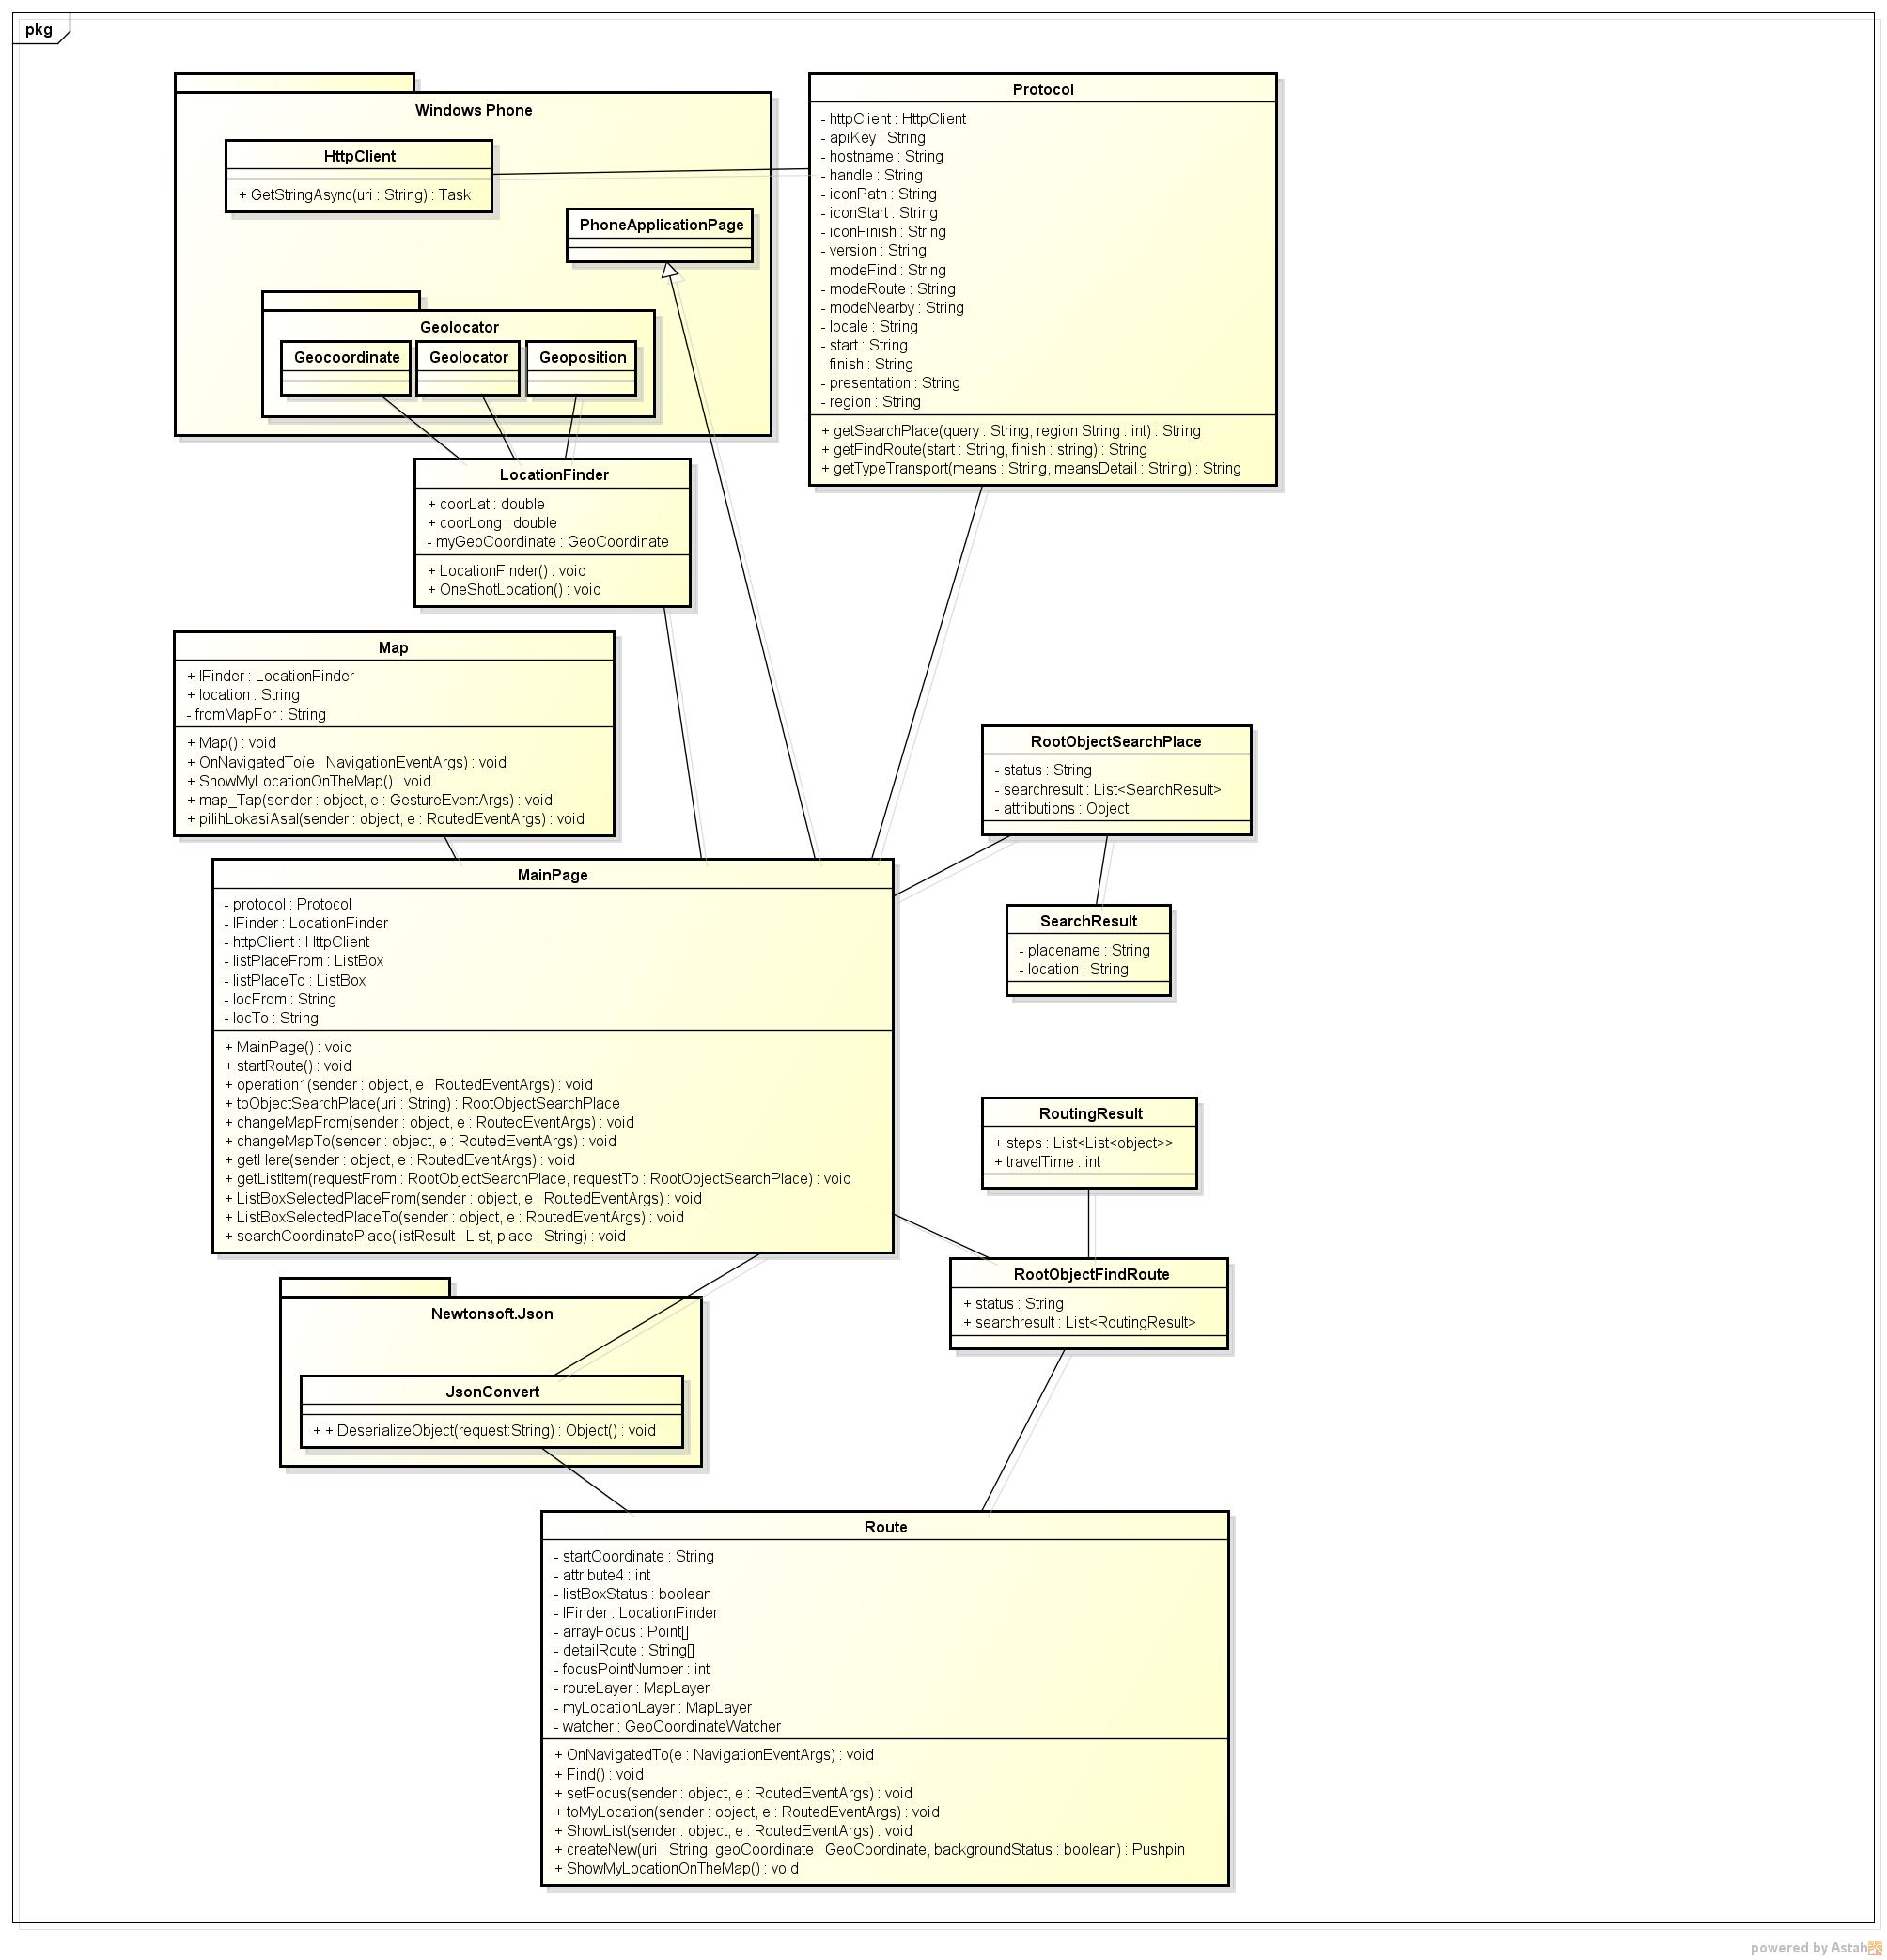
\includegraphics[scale=0.2]{Gambar/useCase_dan_Class/class4}
	\caption{Diagram Kelas}
	\label{fig:kelas}
\end{figure}

%Kelas PhoneApplicationPage
\subsection{Kelas \textit{PhoneApplicationPage}}
\label{lab:Kelas PhoneApplicationPage}
\hspace{0.5cm} \textit{PhoneApplicationPage} merupakan kelas bawaan Windows Phone yang menangani interksi pengguna dengan aplikasi dan siklus hidup aplikasi.

%Kelas MainPage
\subsection{Kelas \textit{MainPage}}
\label{lab:Kelas MainPage}
\hspace{0.5cm} \textit{MainPage} merupakan kelas kelas turunan dari kelas \textit{PhoneApplicationPage} yang menangani interaksi langsung antara halaman aplikasi dengan pengguna. Pada kelas ini akan ditaruh kontrol yang diperlukan. Berikut adalah penjelasan atribut-atribut yang dimiliki kelas ini:
\begin{enumerate}
	\item protocol bertipe Protocol untuk mendapatkan URL yang digunakan dalam permintaan ke Kiri API.
	\item lFinder bertipe LocationFinder yang akan menampung objek untuk pencarian lokasi.
	\item httpClient bertipe HttpClient merupakan objek yang akan mengurus permintaan dan kembalian dari Kiri API.
	\item listPlaceFrom bertipe ListBox untuk menampung dan menampilkan hasil pencarian lokasi terkait dari lokasi awal.
	\item listPlaceTo bertipe ListBox untuk menampung dan menampilkan hasil pencarian lokasi terkait dari lokasi tujuan.
	\item locFrom bertipe string untuk menampung kordinat awal.
	\item locTo bertipe string untuk menampung kordinat tujuan.
	\item centerOfBandung bertipe Point untuk menampung pusat kordinat kota Bandung.
	\item centerOfJakarta bertipe Point untuk menampung pusat kordinat kota Jakarta.
	\item centerOfMalang bertipe Point untuk menampung pusat kordinat kota Malang.
	\item centerOfSurabaya bertipe Point untuk menampung pusat kordinat kota Surabaya.
	\item city bertipe kumpulan String untuk menampung kota yang didukung oleh layanan Kiri.
	\item myCity bertipe String untuk menampung kode kota sesuai Kode Penerbangan IATA.
\end{enumerate}

Berikut adalah penjelasan metode-metode yang dimiliki kelas ini:
\begin{enumerate}
	\item Metode MainPage digunakan sebagai konstruktor pada kelas MainPage. 
	\item Metode startRoute digunakan untuk mendapatkan masukan pengguna lalu mengkalkulasi masukan tersebut menjadi kordinat asal dan tujuan lalu mengirimkannya ke kelas ShowRoute.
	\item Metode toObjectSearchPlace digunakan untuk membuat objek RootObjectSearchPlace dengan masukan uri yang bertipe string.
	\item Metode changeMapFrom digunakan untuk berpindah ke halaman mapFrom.
	\item Metode changeMapTo digunakan untuk berpindah ke halaman mapTo.
	\item Metode getHere digunakan untuk mendapatkan kordinat dimana perangkat berada.
	\item Metode getListItem digunakan untuk membuat listBox lalu menampilkan ke pengguna. 
	\item Metode ListBoxSelectedPlaceFrom digunakan untuk mendapatkan tempat asal yang dipilih pengguna.
	\item Metode ListBoxSelectedPlaceTo digunakan untuk mendapatkan tempat tujuan yang dipilih pengguna.
	\item Metode searchCoordinatePlace digunakan untuk mencari kordinat dari tempat pilihan pengguna.
	\item Metode changeCity digunakan untuk mengubah kota tujuan dari pencarian.
\end{enumerate}

%Kelas Geocoordinate
\subsection{Kelas \textit{Geocoordinate}}
\label{lab:Kelas Geocoordinate}
\hspace{0.5cm} \textit{Geocoordinate} merupakan kelas bawaan dari Windows Phone yang akan dimanfaatkan untuk membaca \textit{latitude} dan \textit{altitude}.

%Kelas Geolocator
\subsection{Kelas \textit{Geolocator}}
\label{lab:Kelas Geolocator}
\hspace{0.5cm} \textit{Geolocator} merupakan kelas bawaan Windows Phone untuk mengkases lokasi. Dengan bantuan kelas ini maka dapat mengetahui status lokasi dari perangkat dan menemukan lokasi secara akurat.

%Kelas Geoposition
\subsection{Kelas \textit{Geoposition}}
\label{lab:Kelas Geoposition}
\hspace{0.5cm} \textit{Geoposition} merupakan kelas yang menampung lokasi sesuak kembalian \textit{Geolocator}.

%Kelas LocationFinder
\subsection{Kelas \textit{LocationFinder}}
\label{lab:Kelas LocationFinder}
\hspace{0.5cm} \textit{LocationFinder} merupakan kelas yang akan menampung lokasi perangkat. Berikut adalah penjelasan atribut-atribut yang dimiliki kelas ini:
\begin{enumerate}
	\item coorLat bertipe Double untuk menampung kordinat latitude.
	\item coorLong bertipe Double untuk menampung kordinat longitude.
	\item myGeoCoordinate bertipe GeoCoordinate untuk menampung lokasi perangkat
\end{enumerate}

Berikut adalah penjelasan metode-metode yang dimiliki kelas ini:
\begin{enumerate}
	\item Metode OneShotLocation\_Click berfungsi inisialisasi GPS lalu mendapat kordinat dan menampungnya di atribut.
\end{enumerate}

%Kelas PointFromMap
\subsection{Kelas \textit{PointFromMap}}
\label{lab:Kelas PointFromMap}
\hspace{0.5cm} \textit{PointFromMap} merupakan kelas yang akan mendapatkan titik yang ditunjuk pengguna pada peta lalu menerjemahkannya dalam bentuk titik kordinat. Berikut adalah penjelasan atribut-atribut yang dimiliki kelas ini:
\begin{enumerate}
	\item latitude
	\item longitude
\end{enumerate}

Berikut adalah penjelasan metode-metode yang dimiliki kelas ini:
\begin{enumerate}
	\item Metode getPoint berfungsi mengambil titik yang ditunjuk lalu menerjemahkan dalam bentuk latitude dan longitude. 
\end{enumerate}

%Kelas HttpClient
\subsection{Kelas \textit{HttpClient}}
\label{lab:Kelas HttpClient}
\hspace{0.5cm} \textit{HttpClient} merupakan kelas bawaan Windows Phone untuk mengatur pengiriman dan kembalian menggunakan protokol HTTP. Berikut adalah penjelasan metode-metode kelas \textit{HttpClient} yang dipakai untuk perancangan aplikasi ini:
\begin{enumerate}
	\item Metode GetStringAsync membutuhkan parameter alamat bertipe string dan mengembalikan kembalian dari Kiri dalam bentuk Task<string>.
\end{enumerate}

%Kelas Protocol
\subsection{Kelas \textit{Protocol}}
\label{lab:Kelas Protocol}
\hspace{0.5cm} \textit{Protocol} merupakan kelas untuk menampung semua alamat dalam pengiriman menggunakan protokol HTTP. Berikut adalah penjelasan atribut-atribut yang dimiliki kelas ini:
\begin{enumerate}
	\item apiKey bertipe string digunakan untuk menyimpan kunci untuk mengirim permintaan ke Kiri.
	\item hostname bertipe string digunakan untuk digunakan untuk menyimpan alamat host dari Kiri.
	\item handle bertipe string digunakan untuk menyimpan alamat host ditambah "handle.php".
	\item iconPath bertipe string digunakan untuk menyimpan lokasi gambar yang dibutuhkan.
	\item iconStart bertipe string digunakan untuk menyimpan lokasi gambar awal perjalanan dari lokasi awal.
	\item iconFinish bertipe string digunakan untuk menyimpan lokasi gambar akhir perjalanan ke lokasi tujuan.
	
	\item version bertipe string digunakan untuk menyimpan veris dari API yang digunakan.
	
	\item modeFind bertipe string yang digunakan untuk menyimpan mode mencari lokasi terkait pada Kiri API.
	\item modeRoute bertipe string yang digunakan untuk menyimpan mode mencari rute pada Kiri API.
	\item modeNearby bertipe string yang digunakan untuk menyimpan mode mencari lokasi terdekat pada Kiri API.
	
	\item locale bertipe string yang digunakan untuk menyimpan kata "locale".
	
	\item start bertipe string yang digunakan untuk menyimpan kata "start".
	\item finish bertipe string yang digunakan untuk menyimpan kata "finish".
	
	\item presentation bertipe string yang digunakan untuk menyimpan kata "presentation".
	
	\item region bertipe string yang digunakan untuk menyimpan kata "region".
\end{enumerate}

Berikut adalah penjelasan metode-metode yang dimiliki kelas ini:
\begin{enumerate}
	\item getTypeTransport merupakan metode yang akan mengembalikan alamat dari gambar transportasi. Metode ini memiliki 2 parmeter yaitu means sebagai tipe transportasi dan meansDetail sebagai nama kendaraan.
	\item getSearchPlace merupakan metode yang akan mengembalikan URI pencarian lokasi sesuai paramater. Parameter yang dimaksud adalah \textit{query} masukan pengguna.
	\item getFindRoute merupakan metode yang akan mengembalikan URI pencarian rute sesuai parameter. Parameter yang dimaksud adalah kordinat lokasi asal dan kordinat lokasi tujuan yang bertipe string.
\end{enumerate}

%Kelas RootObjectSearchPlace
\subsection{Kelas \textit{RootObjectSearchPlace}}
\label{lab:Kelas RootObjectSearchPlace}
\hspace{0.5cm} \textit{RootObjectSearchPlace} merupakan kelas untuk menampung objek hasil pencarian lokasi. Berikut adalah penjelasan atribut-atribut yang dimiliki kelas ini:
\begin{enumerate}
	\item status bertipe \textit{string} digunakan untuk menampung hasil kembalian status dari Kiri.
	\item searchresult bertipe \textit{list} dan menampung banyak objek SearchResult. 
	\item attributions bertipe objek untuk menampung attributions.
\end{enumerate}


%Kelas SearchResult
\subsection{Kelas \textit{SearchResult}}
\label{lab:Kelas SearchResult}
\hspace{0.5cm} \textit{SearchResult} merupakan kelas untuk menampung nama tempat dan kordinat dari nama tempat tersebut. Berikut adalah penjelasan atribut-atribut yang dimiliki kelas ini:
\begin{enumerate}
	\item placename bertipe \textit{string} digunakan untuk menampung nama tempat. 
	\item location bertipe \textit{string} digunakan untuk menampung nama tempat.
\end{enumerate}

%Kelas RootObjectFindRoute
\subsection{Kelas \textit{RootObjectFindRoute}}
\label{lab:Kelas RootObjectFindRoute}
\hspace{0.5cm} \textit{RootObjectFindRoute} merupakan kelas untuk menampung hasil pencarian rute. Berikut adalah penjelasan atribut-atribut yang dimiliki kelas ini:
\begin{enumerate}
	\item status
	\item routingresults
\end{enumerate}

%Kelas RoutingResult
\subsection{Kelas \textit{RoutingResult}}
\label{lab:Kelas RoutingResult}
\hspace{0.5cm} \textit{RoutingResult} merupakan kelas untuk menampung langkah menuju tempat tujuan dan waktu yang dibutuhkan. Berikut adalah penjelasan atribut-atribut yang dimiliki kelas ini:
\begin{enumerate}
	\item steps
	\item traveltime
\end{enumerate}


%Perancangan Antar Muka
\section{Perancangan Antar Muka}
\label{lab:Perancangan Kelas}
\hspace{0.5cm} Pada sub bab ini akan dibahas mengenai antarmuka pada aplikasi Pencari Rute Kendaraan Umum untuk Windows Phone. Antarmuka berfungsi sebagai jembatan yang menghubungkan antara aplikasi dengan pengguna. Berikut ini akan dijelaskan mengenai rancangan antarmuka aplikasi Pencari Rute Kendaraan Umum untuk Windows Phone. 

%Kelas MainPage
\subsection{Antarmuka Kelas \textit{MainPage}}
\label{lab:Antarmuka Kelas MainPage}

% Antarmuka Main
\begin{figure}[h]
	\centering
		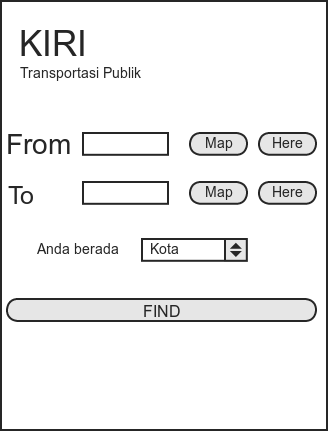
\includegraphics[scale=0.6]{Gambar/perancangan_antarmuka/Home}
	\caption{Antarmuka \textit{MainPage}}
	\label{fig:Antarmuka MainPage}
\end{figure}

\hspace{0.5cm} Antarmuka Kelas Map pada gambar ~\ref{fig:Antarmuka MainPage} merupakan tampilan awal saat aplikasi dijalankan. Antarmuka Kelas Map memiliki dua buah masukan, lima buah tombol, dan satu menu daftar. Berikut adalah detailnya.

Dua buah masukan yaitu.
\begin{itemize}
	\item Masukan lokasi asal\\
	Merupakan masukan lokasi asal mula pengguna ingin melakukan perjalanan.
	\item Masukan lokasi tujuan\\
	Merupakan masukan lokasi tujuan berhentinya perjalanan.
\end{itemize}

Lima buah tombol yaitu. 
\begin{itemize}
	\item Tombol map untuk lokasi asal\\
	Jika tombol ditekan maka akan berpindah ke kelas map untuk memilih lokasi asal di peta. Jika di kelas Map pengguna memilih lokasi maka pada masukan lokasi asal terdapat tulisan "Maps".
	\item Tombol here untuk lokasi asal\\
	Jika tombol ditekan maka lokasi asal adalah lokasi perangkat saat tombol ditekan dan masukan lokasi asal menjadi "here".
	\item Tombol map untuk lokasi tujuan\\
	Jika tombol ditekan maka akan berpindah ke kelas map untuk memilih lokasi tujuan di peta. Jika di kelas Map pengguna memilih lokasi maka pada masukan lokasi tujuan terdapat tulisan "Maps".
	\item Tombol here untuk lokasi tujuan\\
	Jika tombol ditekan maka lokasi tujuan adalah lokasi perangkat saat tombol ditekan dan masukan lokasi tujuan menjadi "here".
	\item Tombol find\\
	Jika tombol ditekan maka akan menampilkan daftar tempat asal dan tempat tujuan lalu mengarahkan ke Kelas Route.
\end{itemize}

Satu buah daftar yaitu.
\begin{itemize}
	\item Daftar kota yang tersedia\\
	Merupkan daftar kota yang tersedia (kota yang rute angkutan umumnya dapat ditemukan dengan aplikasi ini). Disaat aplikasi dijalankan maka daftar akan menunjuk ke kota terdekat tempat perangkat berada.
\end{itemize}

%Kelas Map
\subsection{Antarmuka Kelas \textit{Map}}
\label{lab:Antarmuka Kelas Map}

% Antarmuka Map
\begin{figure}[h]
	\centering
		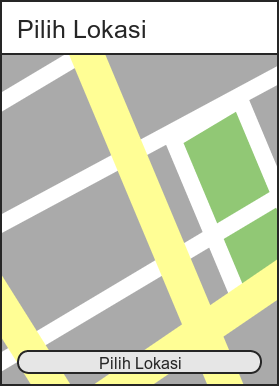
\includegraphics[scale=0.6]{Gambar/perancangan_antarmuka/Map}
	\caption{Antarmuka \textit{Map}}
	\label{fig:Antarmuka Map}
\end{figure}

\hspace{0.5cm} Antarmuka Kelas Map pada gambar ~\ref{fig:Antarmuka Map} merupakan antarmuka untuk menunjuk lokasi pada peta. Terdapat satu buah tombol yang akan dimunculkan jika pengguna sudah memilih lokasi. Jika tombol ditekan maka kordinat lokasi akan di simpan dan dikirim pada kelas MainPage dan halaman akan diarahkan ke kelas MainPage.

%Kelas Route
\subsection{Antarmuka Kelas \textit{Route}}
\label{lab:Antarmuka Kelas Route}

% Antarmuka MapTo
\begin{figure}[h]
	\centering
		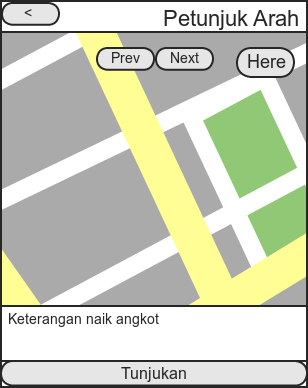
\includegraphics[scale=0.6]{Gambar/perancangan_antarmuka/Route}
	\caption{Antarmuka \textit{Route}}
	\label{fig:Antarmuka Route}
\end{figure}

\hspace{0.5cm} Antarmuka Kelas Route pada gambar ~\ref{fig:Antarmuka Route} merupakan antarmuka untuk melihat rute dari lokasi asal ke lokasi tujuan dalam bentuk daftar maupun peta. Terdapat empat buah tombol pada antarmuka Kelas Route. Berikut tombol yang terdapat pada Kelas Route. 
\begin{itemize}
	\item Tombol prev\\
	Jika tombol ditekan maka akan menunjuk titik sebelumnya pada rute peta.
	\item Tombol next\\
	Jika tombol ditekan maka akan menunjuk titik setelahnya pada rute peta.
	\item Tombol here\\
	Jika tombol ditekan maka akan menunjuk lokasi perangkat berada pada peta.
	\item Tombol Show List\\
	Jika tombol ditekan maka akan menunjuk atau menyembunyikan daftar rute.
\end{itemize}